\documentclass[10pt]{article}

% Lines beginning with the percent sign are comments
% This file has been commented to help you understand more about LaTeX

% DO NOT EDIT THE LINES BETWEEN THE TWO LONG HORIZONTAL LINES

%---------------------------------------------------------------------------------------------------------

% Packages add extra functionality.
\usepackage{
	times,
	graphicx,
	epstopdf,
	fancyhdr,
	amsfonts,
	amsthm,
	amsmath,
	algorithm,
	algorithmic,
	xspace,
	hyperref}
\usepackage[left=1in,top=1in,right=1in,bottom=1in]{geometry}
\usepackage{sect sty}	%For centering section headings
\usepackage{enumerate}	%Allows more labeling options for enumerate environments 
\usepackage{epsfig}
\usepackage[space]{grffile}
\usepackage{booktabs}
\usepackage{amsmath}
\usepackage[super]{nth}
\usepackage{array}

% This will set LaTeX to look for figures in the same directory as the .tex file
\graphicspath{.} % The dot means current directory.

\pagestyle{fancy}

\lhead{\YOURID}
\chead{\MyLang: Language Specification}
\rhead{\today}
\lfoot{CSCI 334: Principles of Programming Languages}
\cfoot{\thepage}
\rfoot{Spring 2022}

% Some commands for changing header and footer format
\renewcommand{\headrulewidth}{0.4pt}
\renewcommand{\headwidth}{\textwidth}
\renewcommand{\footrulewidth}{0.4pt}

% These let you use common environments
\newtheorem{claim}{Claim}
\newtheorem{definition}{Definition}
\newtheorem{theorem}{Theorem}
\newtheorem{lemma}{Lemma}
\newtheorem{observation}{Observation}
\newtheorem{question}{Question}

\setlength{\parindent}{0cm}
%---------------------------------------------------------------------------------------------------------

% DON'T CHANGE ANYTHING ABOVE HERE

% Edit below as instructed
\newcommand{\MyLang}{Panko}	% Replace MyLang with your language name #
\newcommand{\PartnerOne}{Trang Ngo}	% Replace PartnerOne with your name #
\newcommand{\YOURID}{\PartnerOne{}} % Remove \PartnerTwo if working alone.


\title{\MyLang: Language Specification}
\date{Spring 2022}
\author{\PartnerOne{}} % Remove \PartnerTwo if working alone.

\begin{document}
\maketitle

\vspace{\baselineskip}	% Add some vertical space

% Refer to the lab handouts to determine what should go in each of these sections.  Each lab is additive.  So lab 8 should include everything you wrote in lab 7.  Lab 9 should include everything you wrote in lab 8, etc.

\section{Introduction}

    Panko (Paint n Kode) is a drawing language but with a painting twist. Panko allows users to create paintings from individual brush strokes, which are customized by the users. Unlike a drawing language which is more focused on constructing shapes from lines (for example, Logo), Panko aims to create paintings from brush strokes. 
    
     \hspace{}
    
    I think Panko would be a nice addition to the existing drawing programming languages because it aims to create more organic/ painterly paintings. With Panko (and some patience) we can create impressionistic paintings (say, Monet!) using smaller brush strokes of all different colors.
		
\section{Design Principles}

    I would like Panko to be simple and intuitive so that users
    without a background in programming could create artworks with Panko. The design for Panko should be somewhat similar to other drawing languages with coordinate board. However, since Panko's users are building the painting from brush strokes, Panko should definitely has support for loops and lists. 
    
    \hspace{}
    
    I would also like to introduce some intended randomness/ unpredictability into the language. There will be "magic numbers" that users can add to a specific brush stroke so that when being "painted" multiple times, the brush strokes (although of the same "type") turn out a bit different. I think this will encourage the users to experiment more with the language and also mimic the trial and error aspect of the physical painting experience.

\section{Example Programs}

    Example 1: Abstract painting with only one type of rectangle brush stroke of one color. 
    
\begin{verbatim}
canvas = Canvas(800, 800, color = white)
# create the rectangle brush stroke 
rectStroke = Stroke(shape = rectangle, length = 20px, width = 5px, color = purple)
for x in range(0,800, step = 30) 
    for y in range(0, 800, step = 10)
        paint(rectStroke, coord = (x,y))
\end{verbatim}

    Example 2: Abstract painting with one type of round brush but different colors. 
    This painting will have 15 dots of each of the seven rainbow colors located randomly on the page. 
    
\begin{verbatim}
canvas = Canvas(800, 800, color = black)
# create the round brush stroke 
roundStroke = Stroke(shape = circle, radius = 20px)
rainbow = [red, orange, yellow, green, blue, indigo, purple]
for color in rainbow
    for i in range(0, 15, step = 1) 
        x = random(0,800)
        y = random(0,800)
        paint(roundStroke, coord = (x,y), color = color)
\end{verbatim}

    Example 3: A painting of a flower field - this example makes use of the intended randomness to transition between colors. The \texttt{color} argument is given a tuple. The color of the dots will be a random color \emph{between} the two specified colors.
    
\begin{verbatim}
# a square 800x800px canvas
canvas = Canvas(800, 800, color = sageGreen)
# create a round stroke but with random radius
randomRoundStroke = Stroke(shape = circle, radius = 20px)
#create a painting of a flower field using the newly created strokes
for _ in range(0,100)
    paint(randomRoundStroke, coord = ( random(0,800), random(0,800)), 
    color = (pink, blue))
\end{verbatim}
    
\section{Language Concepts}

    In order to write programs using Panko, a user needs to understand the coordinate board and how to specify location with coordinates. They also need to understand the necessary features of a brush stroke (color, location, shape, size) and how to specify them with the appropriate units. 

\section{Syntax}

    A program written in Panko creates a \emph{painting}. A  \emph{painting} consists of: 
    
    -  \emph{Canvas}: the background of the painting, which consists of:
    
    +  \emph{Size}
    
    +   \emph{Color} 
    
    - A collection of brush strokes (zero or more). Each brush stroke consists of: 
    
    + \emph{Name}
    
    +  \emph{Shape}, which consists of a few predefined types: rectangle, circle, curve, square. Each of these types consist of their size (length and width or radius).
    
    +  \emph{Color}
    
    Here is the minimal formal grammar in BNF form:
    \begin{verbatim}
    <painting>    ::= <canvas><brushstroke>
    <canvas>      ::= <width><height>
    <brushstroke> ::= <name><shape><color>
    <shape>       ::= <rectangle>
    <rectangle>   ::= <width><height>
    <color>       ::= <hex><hex><hex><hex><hex><hex>
    <width>       ::= int 
    <height>      ::= int
    <name>        ::= string 
    <hex>         ::= 0 | 1 | 2 | 3 | 4 | 5 | 6 | 7 | 8 | 9 
                    | a | b | c | d | e | f 
    \end{verbatim}

\section{Semantics}

\begin{enumerate}
    \item 
    \emph{What are the primitive kinds of values in your system? For example, a primitive might be a
number, a string, a shape, a sound, and so on. Every primitive should be an idea that a user
can explicitly mention in a program.}

    Primitives in Panko can be brush strokes, which consist of a shape and a color. Note that when declaring a brush stroke users do not have to also specify the location of the stroke yet. 
    
    \item 
    \emph{What are the “actions” or compositional elements of your language? In other words, how are
values combined? For example, your system might combine primitive “numbers” using an
operation like “plus.” Or perhaps a user can arrange “notes” in a “sequence.”}

    The main command in Panko is \texttt{paint} which takes a brush stroke and location (specified in x, y coordinate). \texttt{paint} puts the specified brush stroke at the specified location. 
    
    \item 
    \emph{How is your program represented? In other words, what components (types) will be used in
your AST? If it helps you to think about this using ML algebraic data types, please use them.
Otherwise, a rough sketch like a class hierarchy drawings or even a Java class file is OK.}

    A shape can be represented as a tuple of integers, where the integers represent the measurements of the shape. For example, for a rectangle or a square we only need the length and width. For a circle we will only need to radius.
    
    A color is a hex string. 
    
    A brush stroke can be represented as a tuple of \emph{name} (which is saved as a variable), \emph{shape} and \emph{color}. Note that without the name we will not be able to \texttt{paint} the brush stroke onto the canvas. 

    \item 
    \emph{How do AST elements “fit together” to represent programs as abstract syntax?  For the three
example programs you gave earlier, provide sample abstract syntax trees.}

    Sample ASTs for the three examples above:
    
    Example 1: 
    
     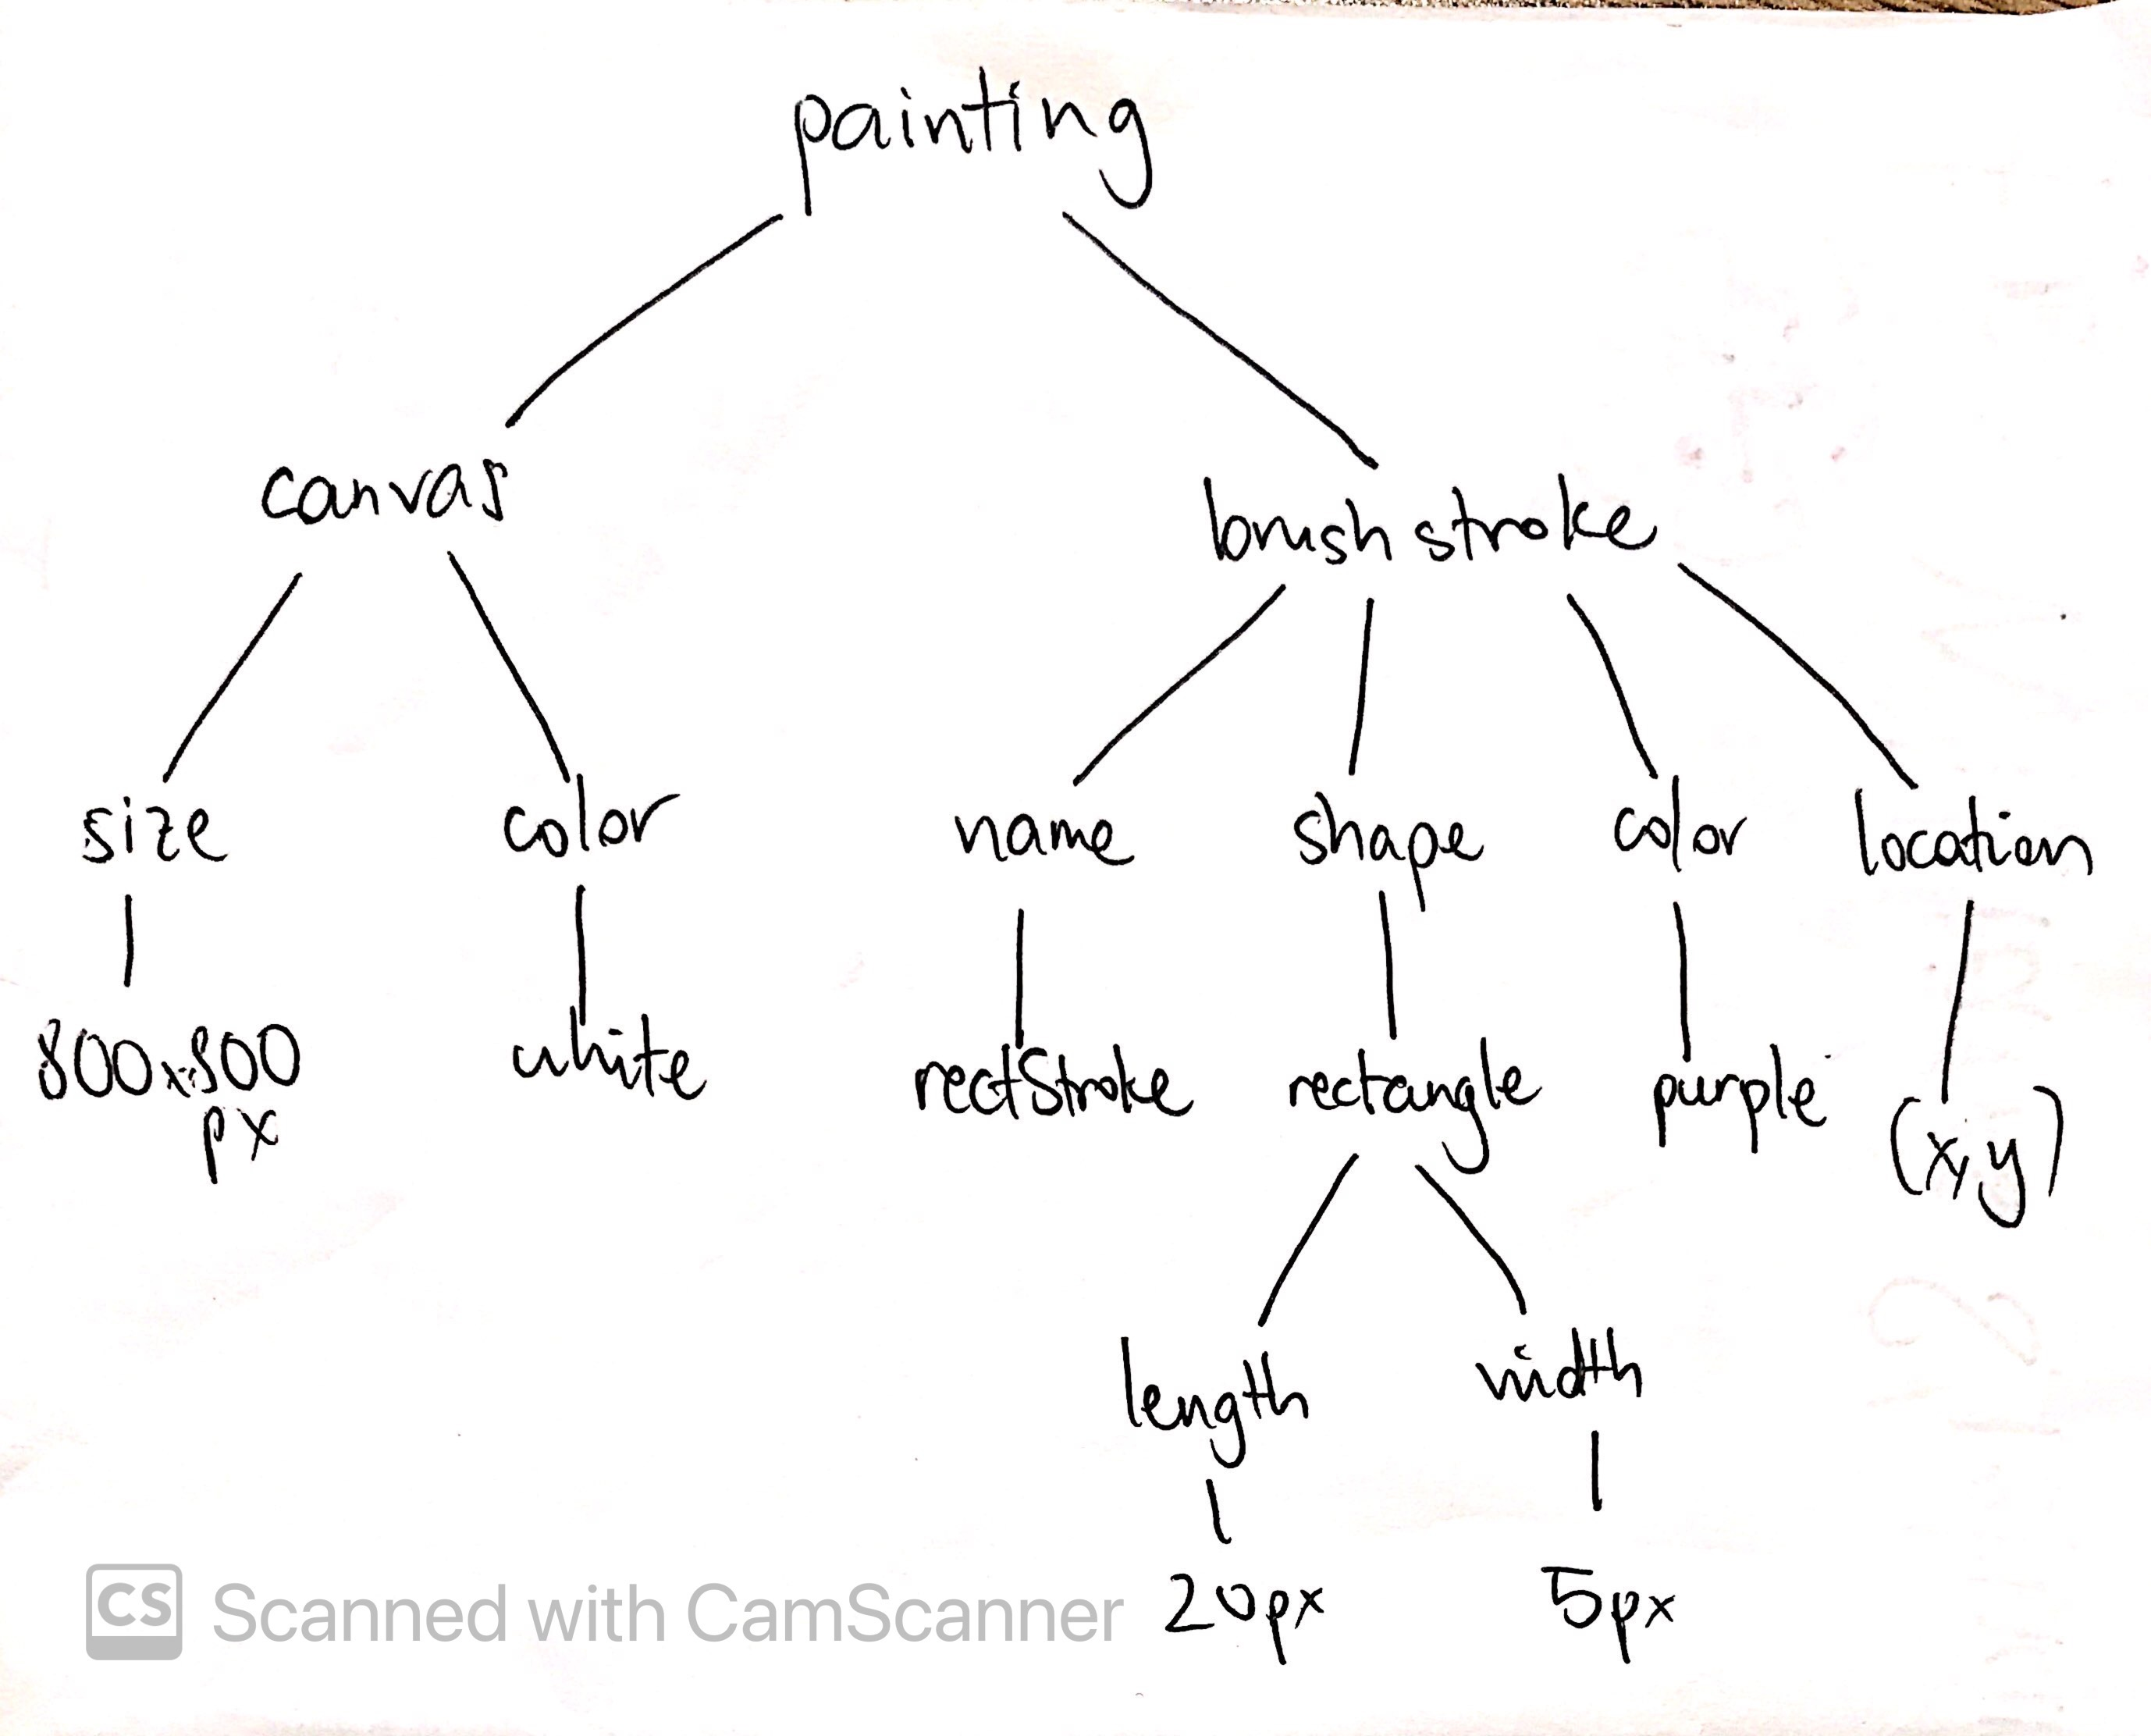
\includegraphics[scale=0.1]{./eg1.jpg}
    
    Example 2:
    
     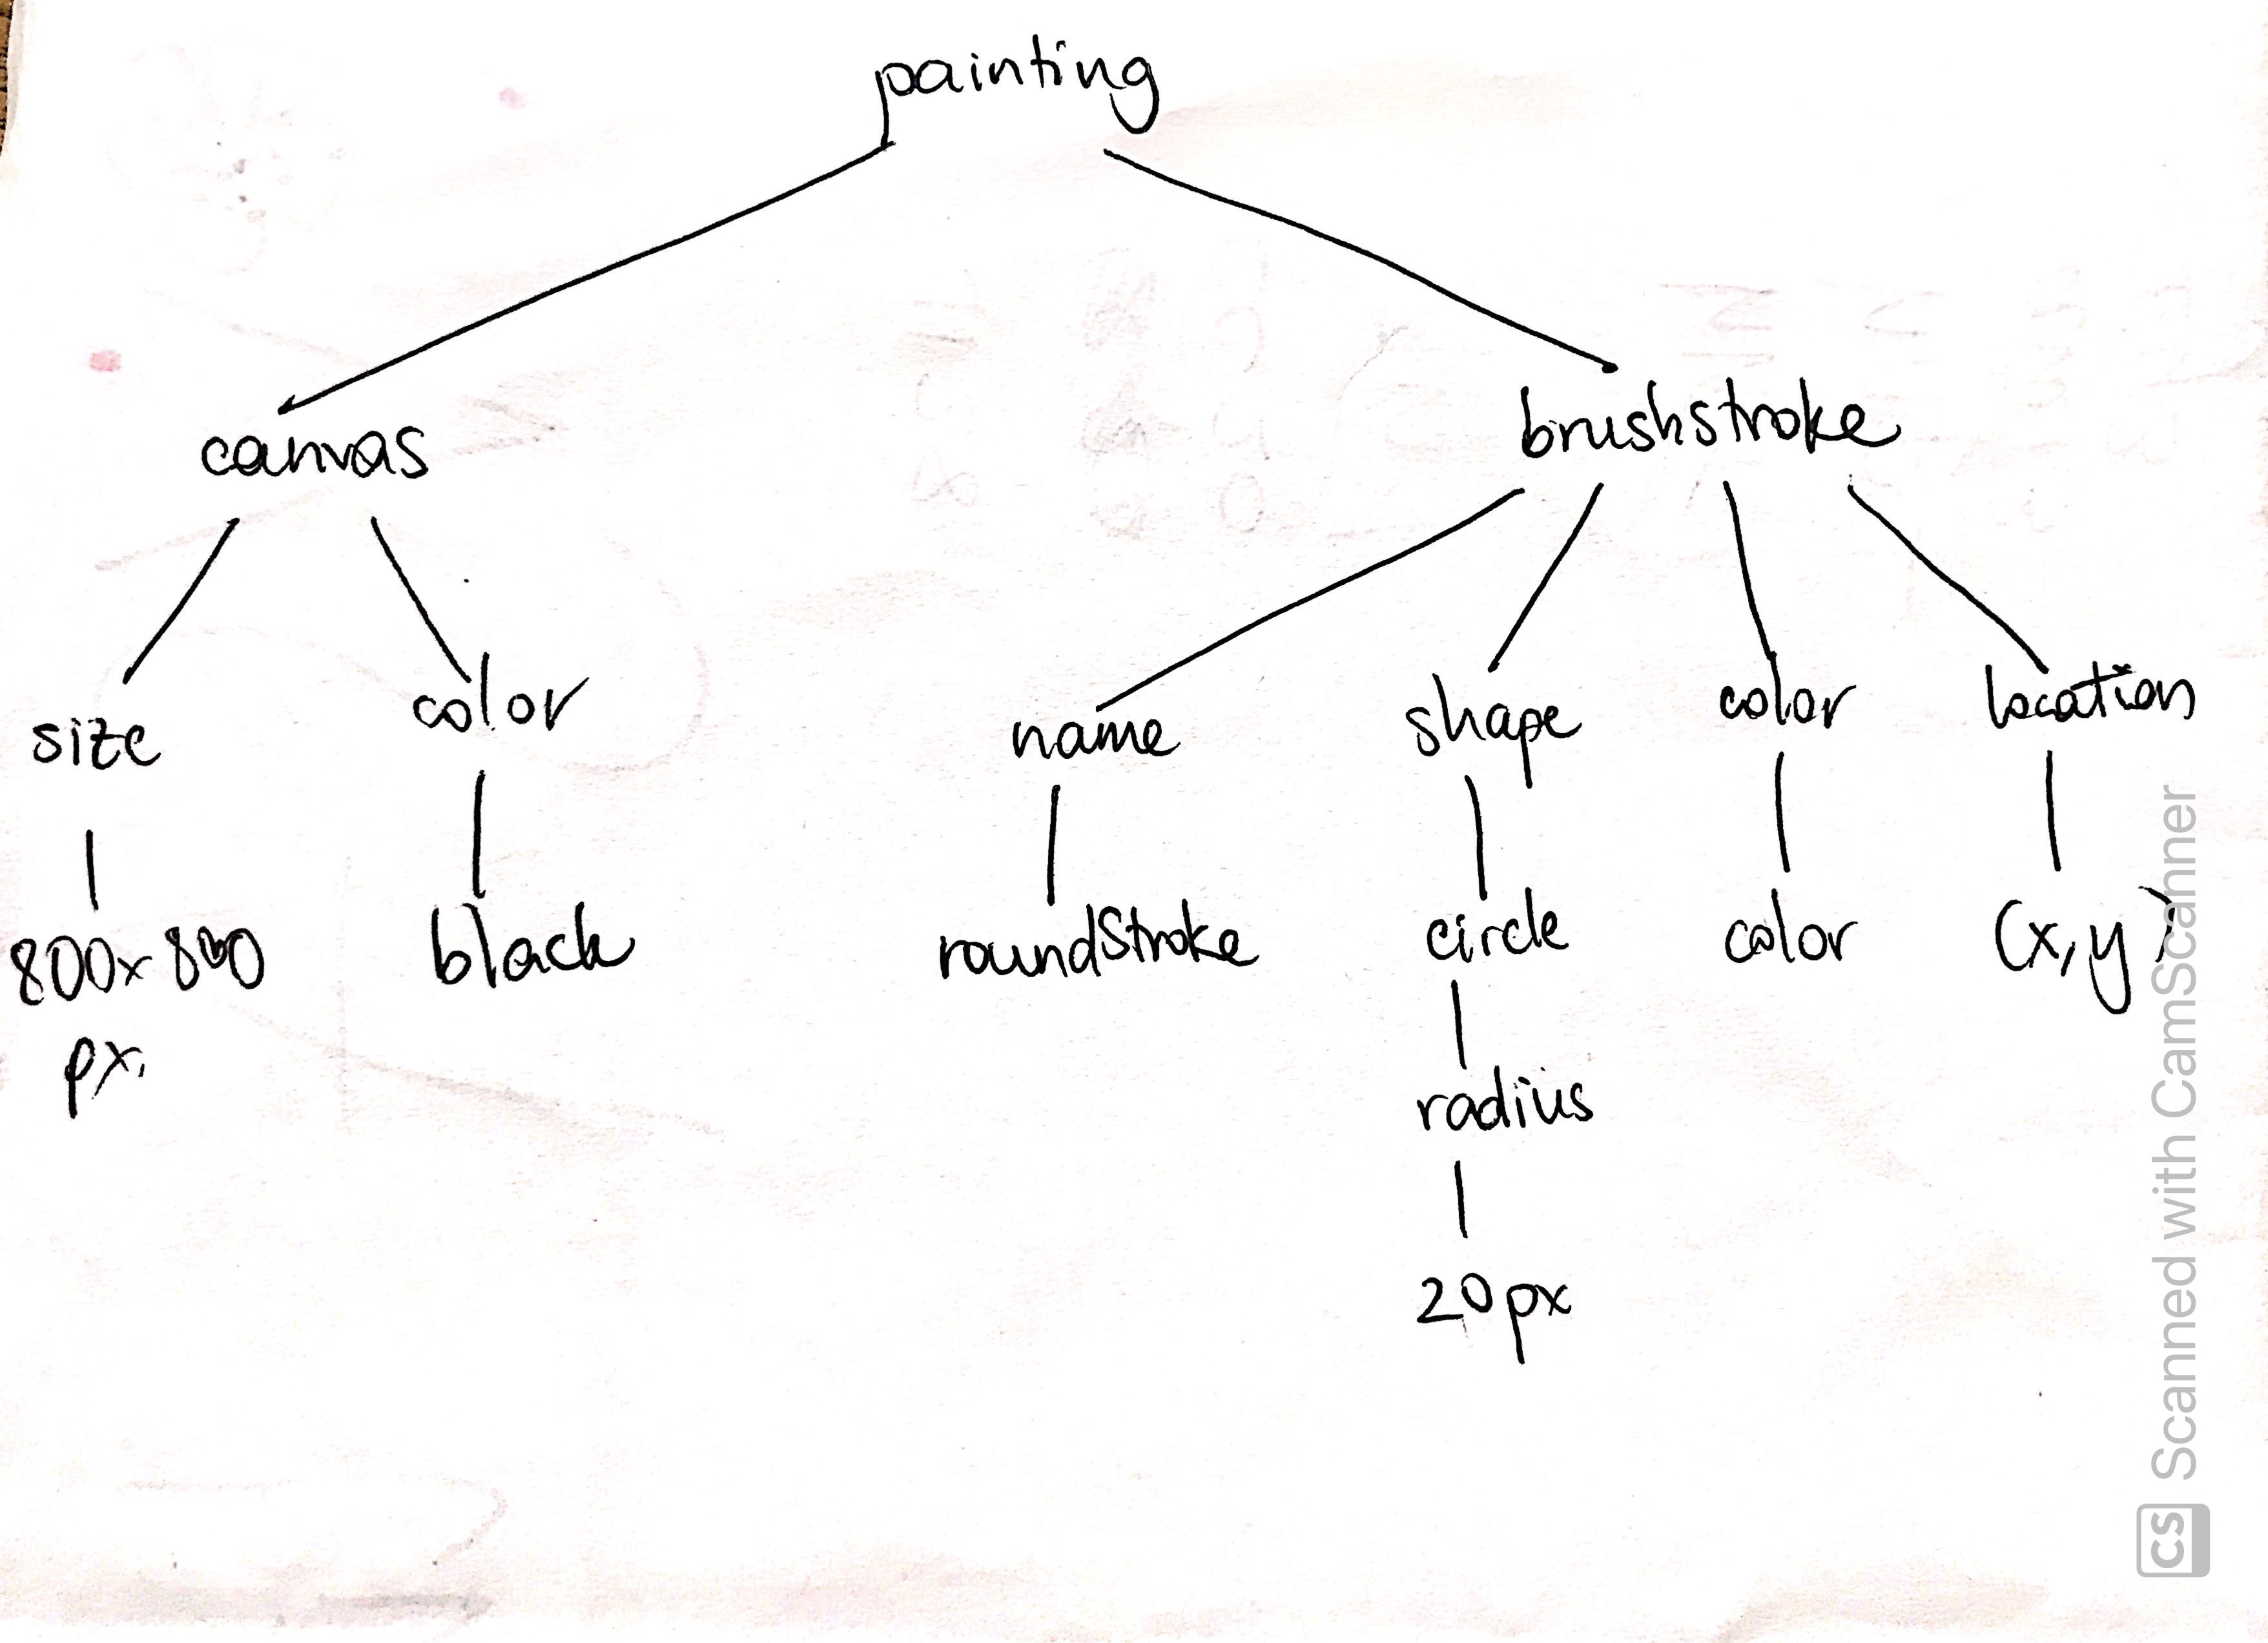
\includegraphics[scale=0.1]{./eg2.jpg}
    
    Example 3:
    
     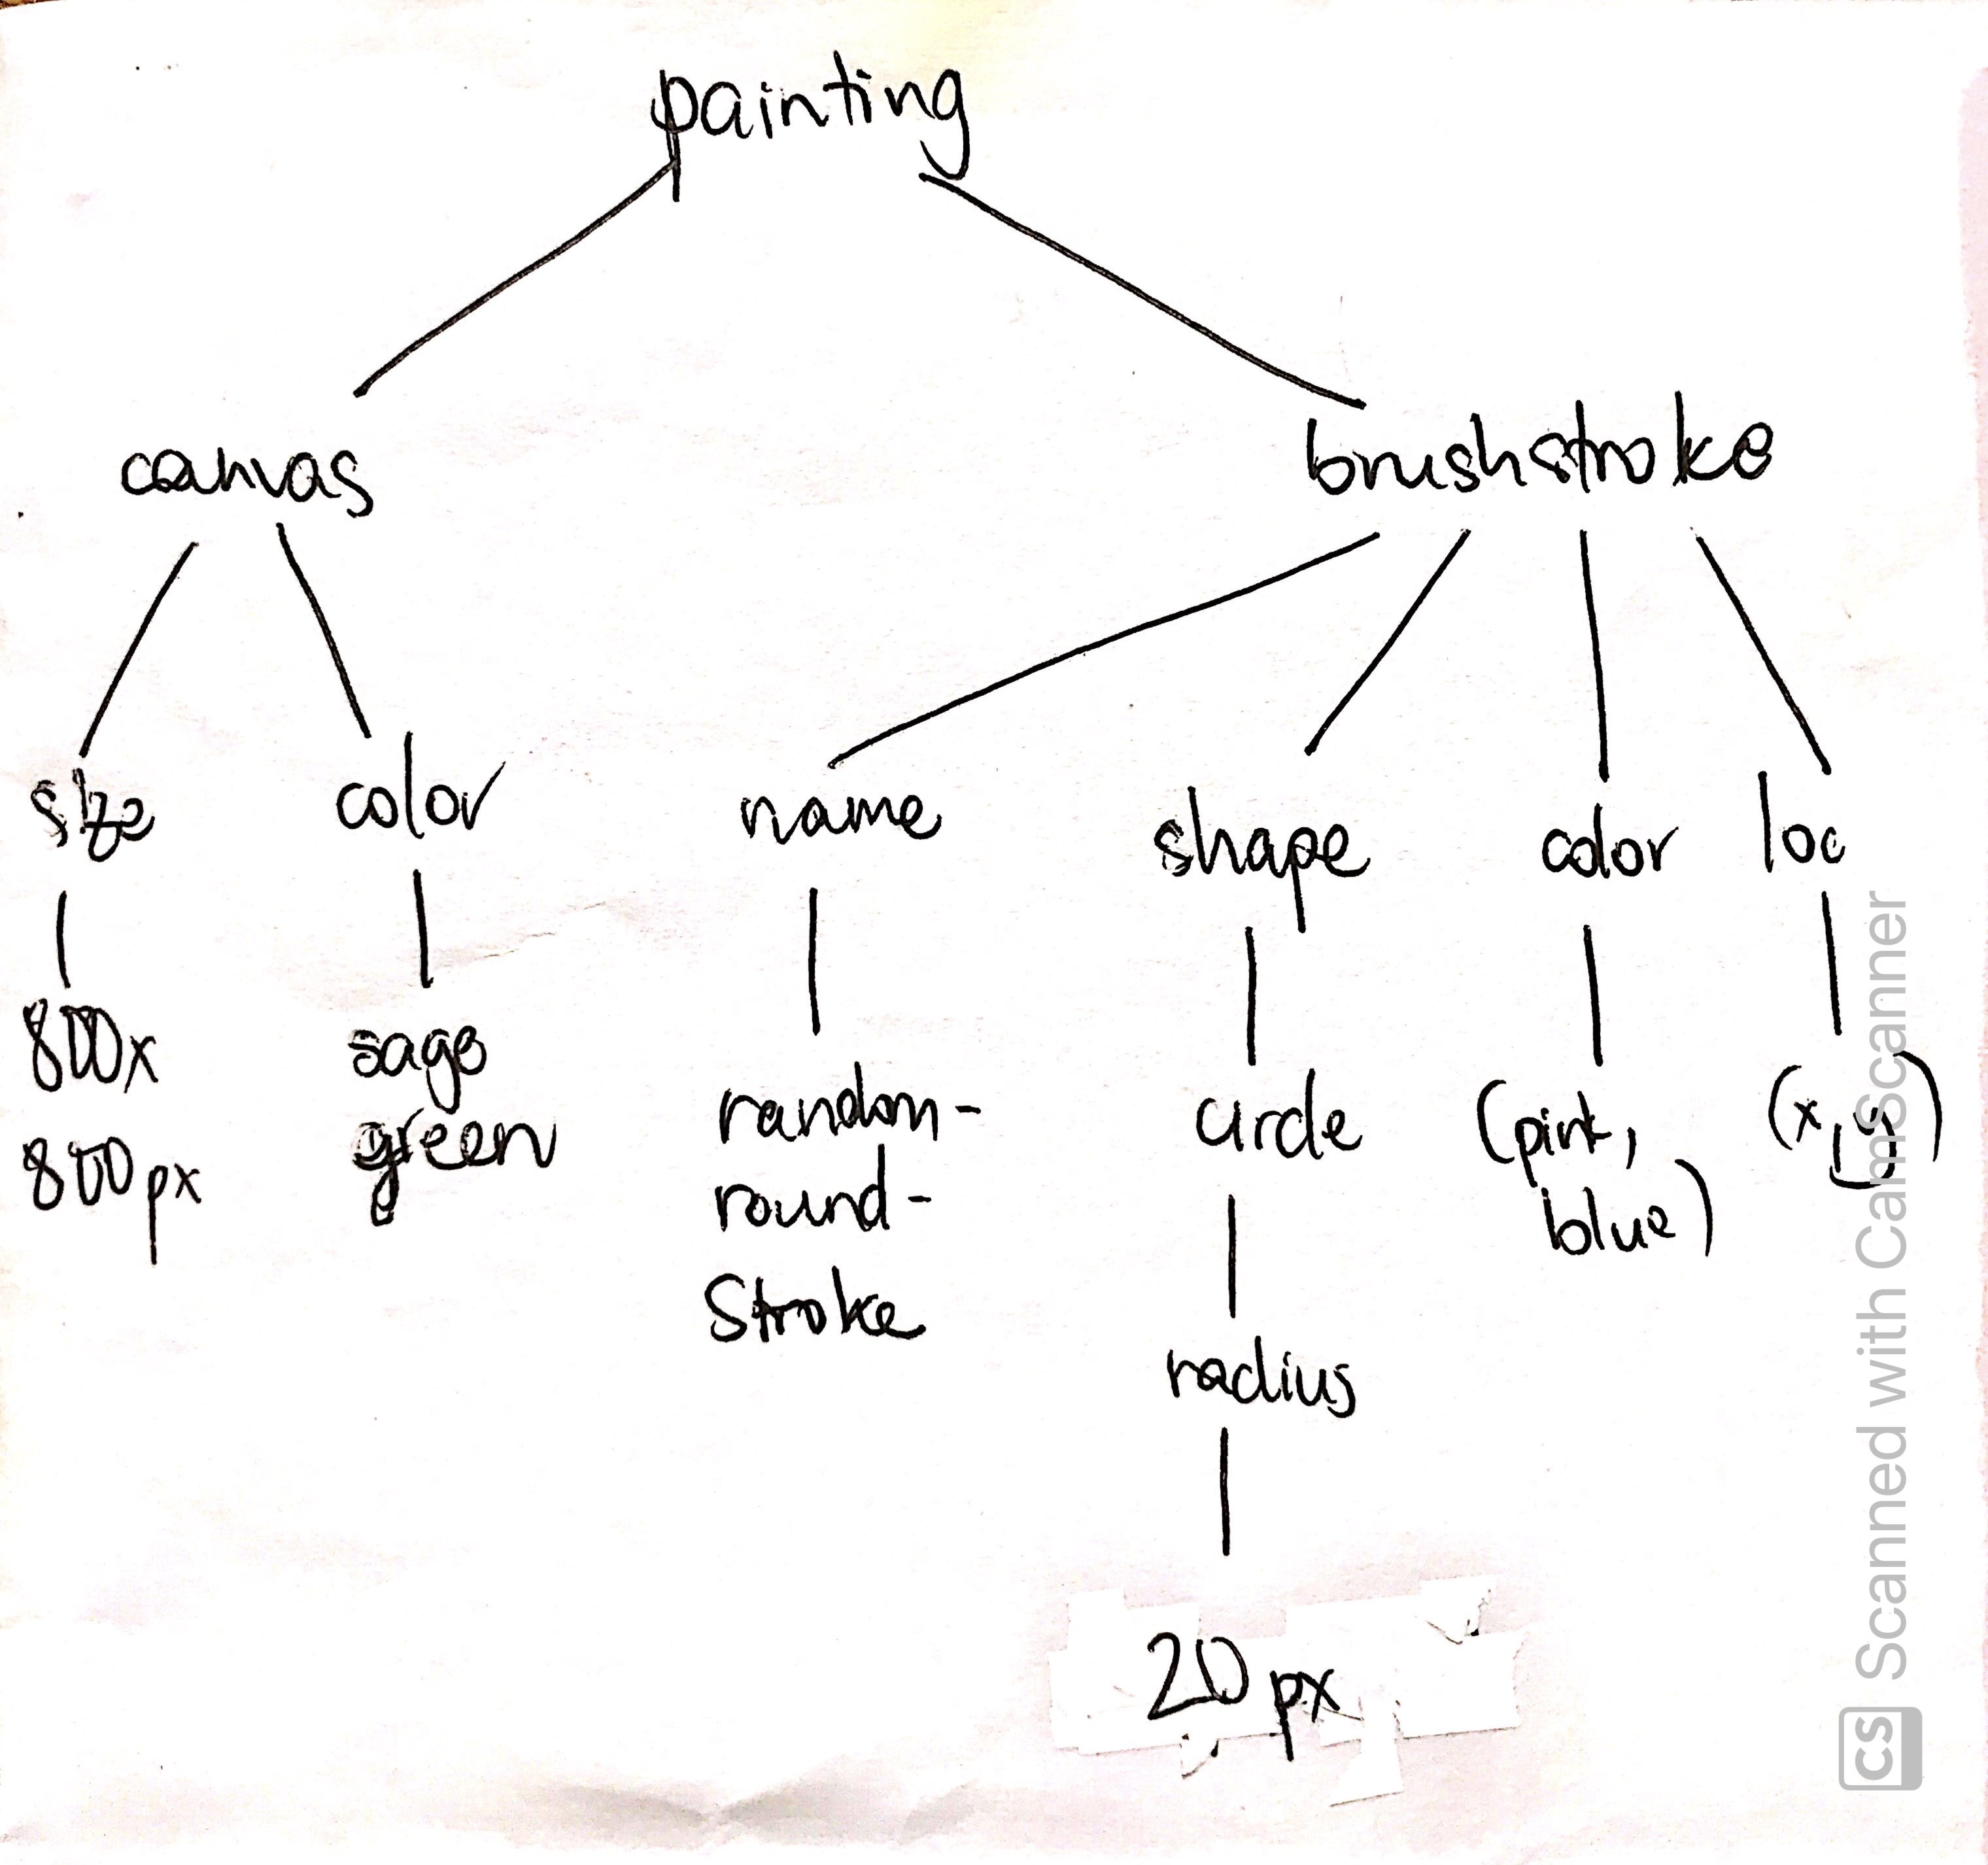
\includegraphics[scale=0.1]{./eg3.jpg}
    
    \item
    \emph{How is your program evaluated? In particular,}
    
    \begin{enumerate}
        \item \emph{Do programs in your language read any input?}
        
        Programs written in Panko do not take any extra input. 
        
        \item \emph {What is the effect (output) of evaluating a program?}
        
        The output is the painting created by the user. It will be a pdf file. 
        
        \item \emph{Evaluation is usually conceived of as a post-order traversal of an AST. Describe how
such a traversal yields the effect you just described and provide illustrations for clarity.
Demonstrate evaluation for at least one of your example programs.}

   A post-order traversal of an AST would yield a painting (which is a collection of brush strokes on top of a canvas). Evaluation for example 1:
   
   Recall the AST for the first example is:
   
   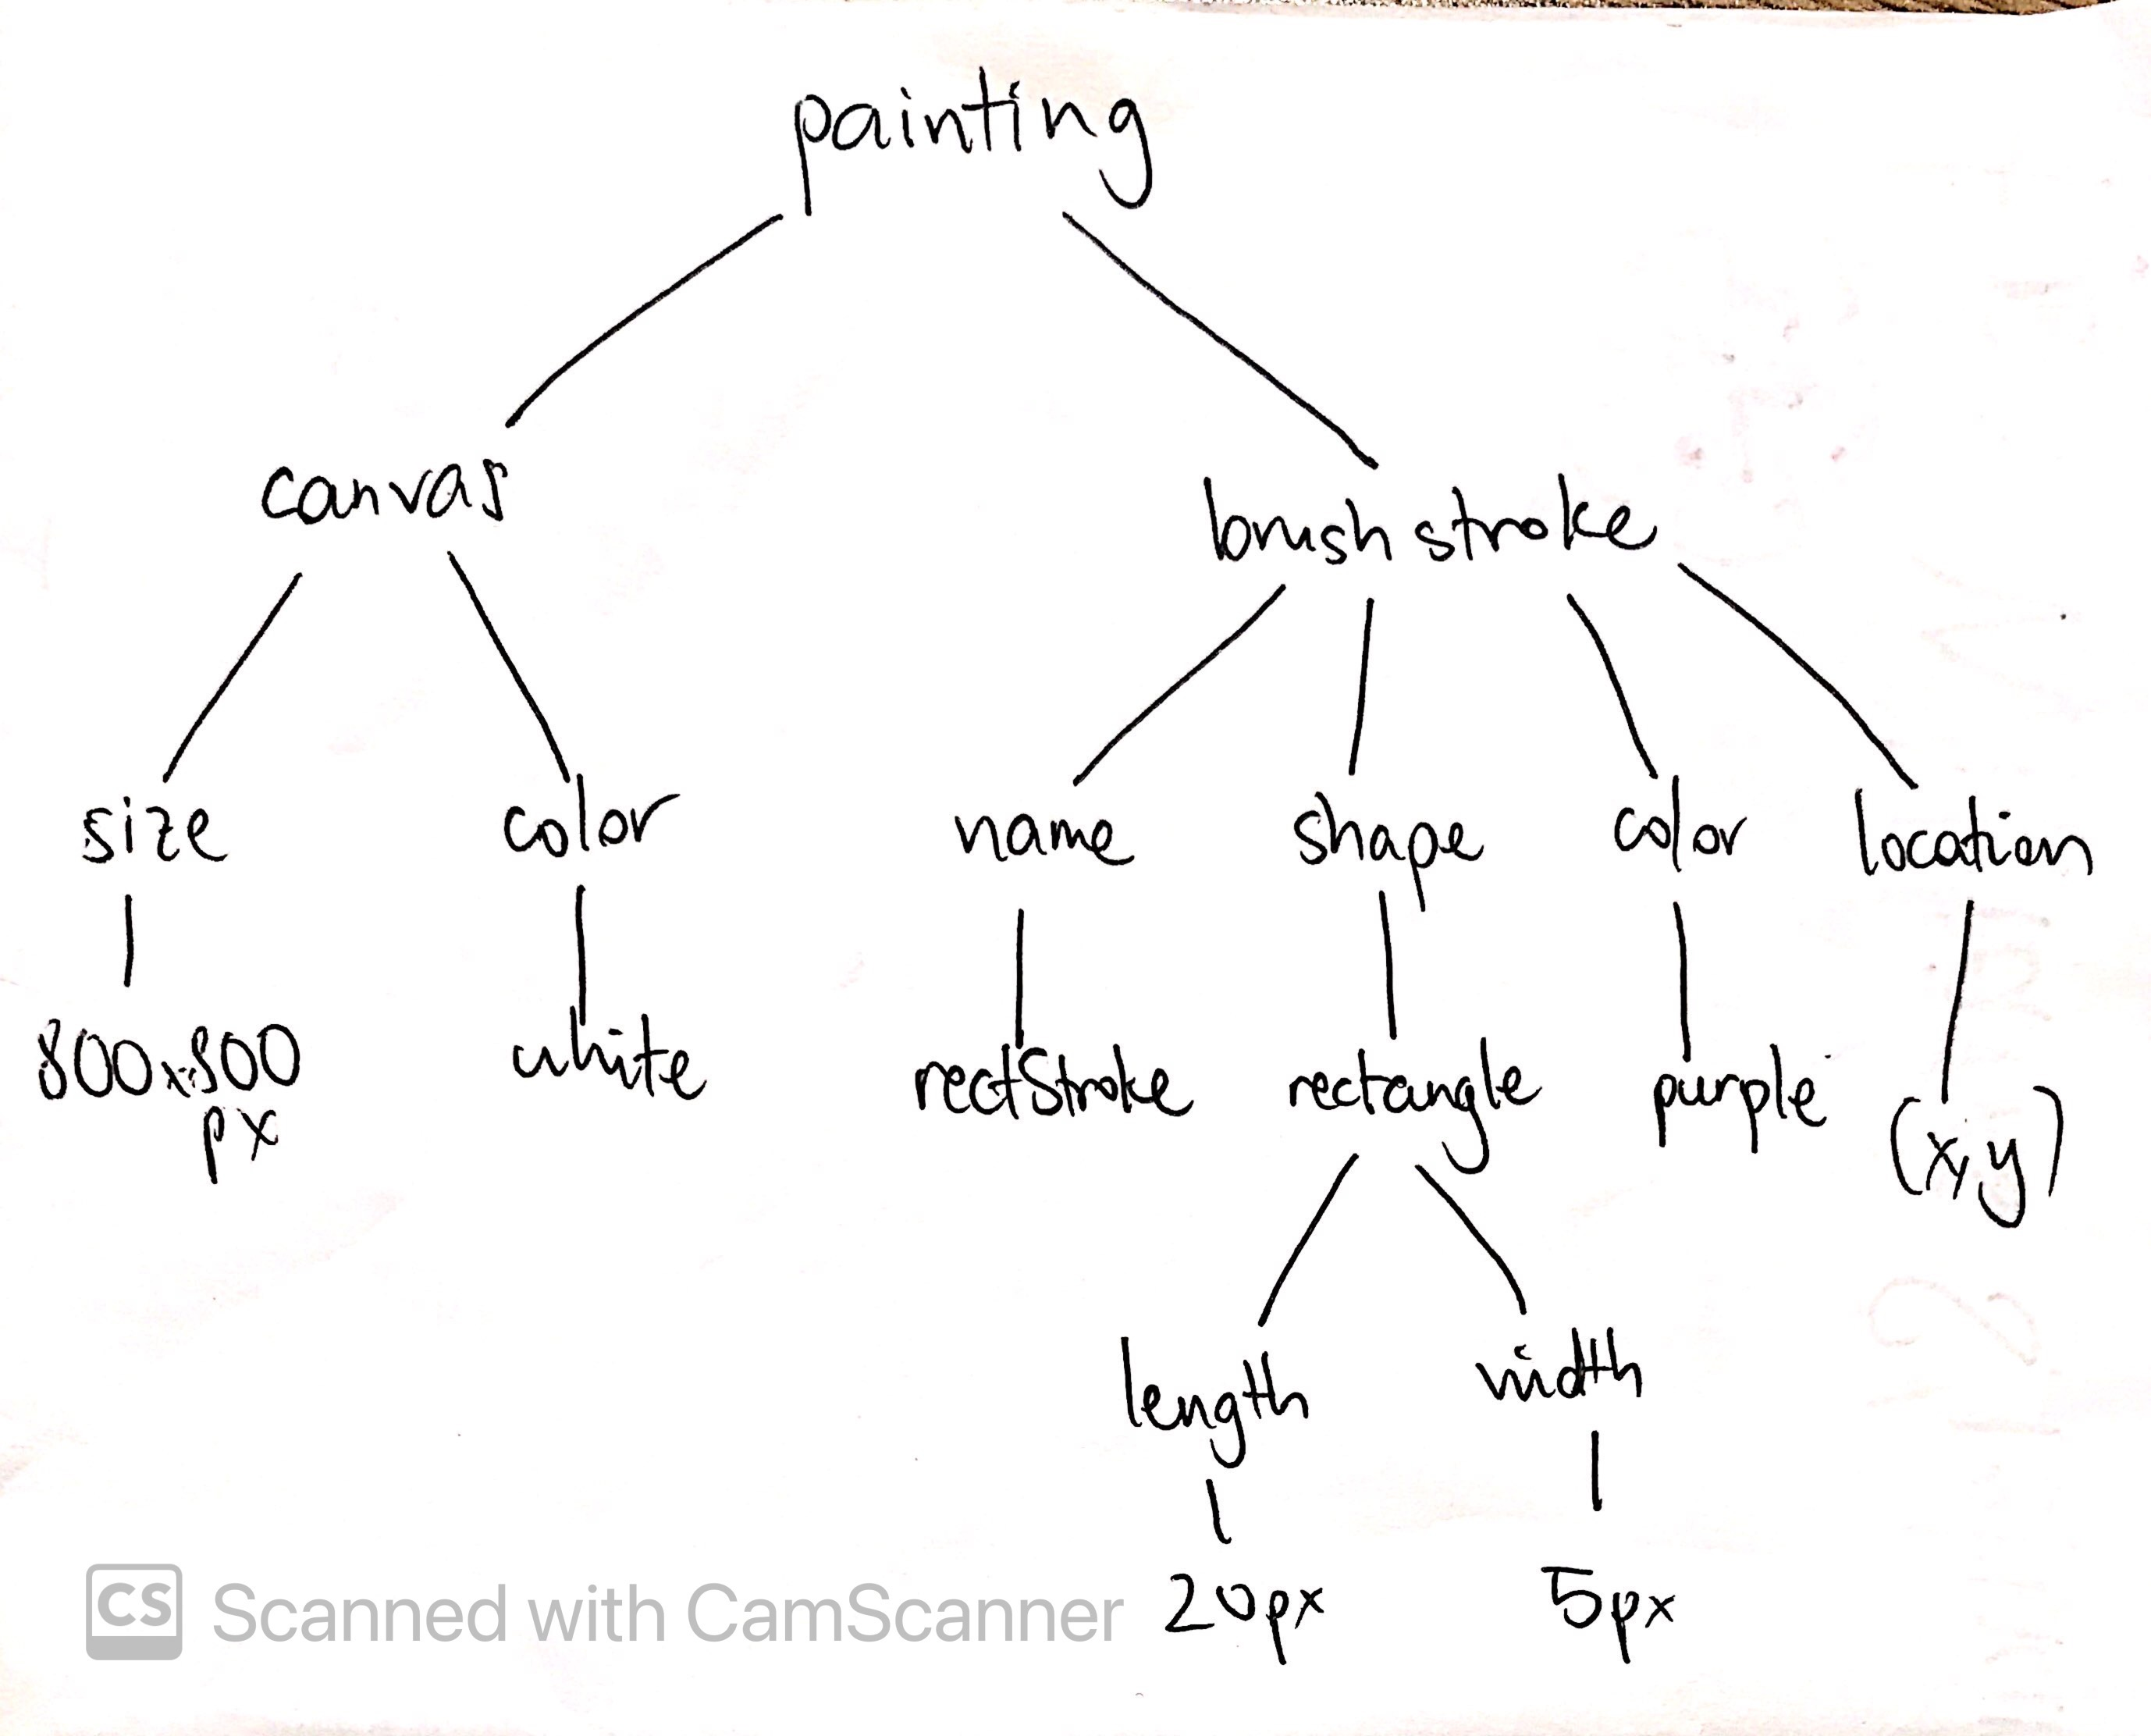
\includegraphics[scale=0.06]{./eg1.jpg}
   
   - First, the canvas subtree would be evaluated. Note that the brush strokes' location depends on the fact that the canvas size has been evaluated. 
   
   - The length and width of the rectangle shape would then be evaluated. 
   
   - With the shape and other features defined, the brush stroke declaration can then be evaluated. 
   
   Note that the location is written as a branch of the brush stroke, but in fact, location is not needed when creating a brush stroke. location is actually an argument of the \texttt{paint} function. This allows users to \texttt{paint} one brush stroke (by referring to its name) at multiple different locations, and also supports the use of for loops.
   
   - With both canvas and brush strokes evaluated, the program can produce the final painting. 
   
    \end{enumerate}
    
        Minimal semantics of Panko:

\begin{table}[bp!]
        \begin{tabular}{|p{3cm}|p{2.5cm}|p{2cm}|p{2cm}|p{4cm}}
        \textbf{Syntax} & \textbf{Abstract Syntax} & \textbf{Type} & \textbf{Prec./Assoc.} & \textbf{Meaning} \\
        \hline
        n & n of int & int & n/a & n is a primitive, a positive integer. It is used to define the width and height of certain brush strokes and canvas. \\
        \hline 
        canvas(width, height) & Canvas of Width*Height & int * int & There should only be one at the beginning of the file. & Canvas is a primitive. It defines the outer bound of the painting, which is a rectangle of width and height. \\
        \hline
        stroke(rectangle (width, height), color = 6ac6bc) & BrushStroke of Shape*Color & (int * int) * string & n/a & A brush stroke is a primitive. It has a shape and color. In the minimal working example, the only possible shape is a rectangle. \\
        \hline 

        \end{tabular}
        \caption{\label{tab:table-name}Minimal semantics of Panko.}
\end{table}
    
\end{enumerate}

% DO NOT DELETE ANYTHING BELOW THIS LINE
\end{document}